\documentclass[12pt]{article}

\usepackage{amsmath}
\usepackage{gensymb}
\usepackage{graphicx}

\graphicspath{ {./images/} }

\begin{document}

\title{Activity II: Earth, Moon, and Some Basic Physics}

\maketitle

\section{Introduction and Objective}

In this activity you will work in groups to answer the following questions regarding the Earth, the Moon, and some basic physics.\newline
\flushleft{$essential$ $concepts$\newline}

For each statement, circle or fill in the blank with the most appropriate term(s).\newline


\begin{enumerate}
        \item A planet that has a perfectly circular orbit has an eccentricity of \underline{0}.
        \item The Ptolemaic model of the Solar System employed a complex series of  deferents and epicycles to explain \underline{planetary motion}.
        \item Light is a wave, but it is also a \underline{particle} according to the explanation of blackbody radiation by Max Planck (and Albert Einstein).
        \item When waves overlap, they combine \underline{constructively} or \underline{destructively}.
        \item When the Moon is becoming more visible over the course of its revolution around Earth, we refer to this as \underline{waxing}.
        \item Stellar parallax can be used to determine the distances to only \underline{relatively close stars}.
        \item The most abundant element in Earth’s atmosphere is \underline{Nitrogen}.
        \item The symbol $T$ refers to the \underline {period} of a wave or orbit.
        \item The symbol $\lambda$ refers to the \underline{wavelength} of a wave.
        \item Planets that orbit farther from the Sun take \underline{more} time to complete one orbital period, which is a consequence of \underline{Kepplers second law}.
        \item The heliocentric model of the Solar System can explain \underline{phases} of Venus, which the Ptolemaic model cannot explain.
        \item The equation $c = \lambda f$ implies that light of high frequency has a \underline{small wavelength}.
        \item The blackbody curve physicists derived in the 19th century is called \underline{Rayleigh Jeans law} and it predicted that the intensity of blackbody radiation for small wavelengths should be infinity.
        \item The prediction referred to in the previous problem (that the intensity of light emitted by a blackbody approaches infinity for small wavelengths) is called \underline{ultraviolet catastrophe}

\end{enumerate}
$open-ended$ $questions$

        \begin{enumerate}
                \item The red giant Betelgeuse has a parallax angle of about 4.5 × $10^{-3}$ arcseconds. About how far away is it, in light years? What is its parallax angle in degrees?

                    \begin{equation}
                        distance = \frac{1}{\theta}
                    \end{equation}

                    \begin{equation}
                        distance = \frac{1}{\left(\frac{1}{4500}\right)^{\circ} \times \frac{\pi}{180}}
                    \end{equation}

                    
                    \begin{equation}
                        distance = \frac{810000}{\pi}
                    \end{equation}

                    \begin{equation}
                        distance = \frac{810000}{\pi}
                    \end{equation}
                    
                    \begin{equation}
                        distance = 257831 \text{ AU} = 4.07 \text{ light-years}
                    \end{equation}

                    The parallax angle is 4.5 \times $10^{-3}$ which is \newline
                    \begin{equation}
                        \left(\frac{1}{4500}\right)^{\circ}
                    \end{equation}

                \item Suppose you are using stellar parallax to determine the distances to stars. Will the stars that have the smallest parallax angles be the closest or farthest stars? Draw a diagram to illustrate.\newline
                    Closer stars will have larger parallax angle and farther stars will have smaller parallax angle.\newline\newline
                    \centerline{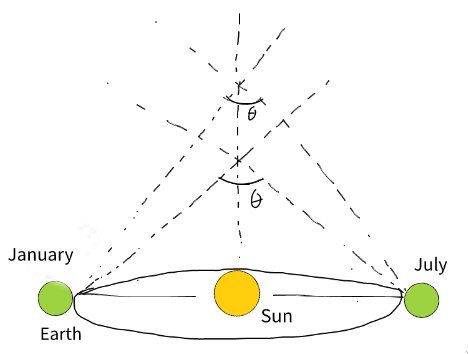
\includegraphics[scale=0.5]{illustration}\newline}
                    As you can imagine, the farther the star, the tighter the angle.

                \item State and describe three ways that our atmosphere protects and incubates life on Earth.
                    \begin{enumerate}
                        \item The earths atmosphere blocks X-rays, Gamma rays and ultraviolet light, which are very harmful to us.
                        \item The greenhouse effect keeps earths surface temperature at a comfortable level where life can thrive.
                        \item Convection creates wind and weather. Which life needs in order to survive. Like how plants need rain water. 
                    \end{enumerate}


        \end{enumerate}

————————————————

\end{document}
